% ==============================================================================
% EURECOM - Cryptography Project Presentation
% PUDA: Private User Data Aggregation for Federated Learning
% ==============================================================================

\documentclass[aspectratio=169,10pt]{beamer}

% ==============================================================================
% PACKAGES
% ==============================================================================
\usepackage[utf8]{inputenc}
\usepackage[T1]{fontenc}
\usepackage{lmodern}
\usepackage{amsmath,amssymb,amsthm}
\usepackage{mathtools}
\usepackage{tikz}
\usepackage{pgfplots}
\usepackage{booktabs}
\usepackage{listings}
\usepackage{xcolor}
\usepackage{graphicx}
\graphicspath{{figures/}}
\usepackage{hyperref}
\usepackage{colortbl}

\usetikzlibrary{arrows.meta,positioning,shapes.geometric,calc,decorations.pathreplacing,backgrounds,fit}
\pgfplotsset{compat=1.18}

% ==============================================================================
% COLORS
% ==============================================================================
\definecolor{bglight}{RGB}{255,255,255}
\definecolor{textdark}{RGB}{40,40,50}
\definecolor{textmuted}{RGB}{100,100,115}
\definecolor{primary}{RGB}{0,90,160}
\definecolor{secondary}{RGB}{120,60,150}
\definecolor{accent}{RGB}{0,140,140}
\definecolor{success}{RGB}{40,160,80}
\definecolor{warning}{RGB}{200,120,0}
\definecolor{danger}{RGB}{200,60,60}
\definecolor{codebg}{RGB}{248,248,252}

% ==============================================================================
% BEAMER THEME
% ==============================================================================
\usetheme{default}
\setbeamercolor{background canvas}{bg=bglight}
\setbeamercolor{normal text}{fg=textdark}
\setbeamercolor{frametitle}{fg=primary,bg=bglight}
\setbeamerfont{frametitle}{size=\large,series=\bfseries}
\setbeamercolor{title}{fg=primary}
\setbeamercolor{subtitle}{fg=secondary}
\setbeamercolor{structure}{fg=primary}
\setbeamercolor{itemize item}{fg=primary}
\setbeamercolor{itemize subitem}{fg=secondary}
\setbeamertemplate{itemize item}{\small$\bullet$}
\setbeamertemplate{itemize subitem}{\small$\circ$}
\setbeamercolor{block title}{fg=white,bg=primary}
\setbeamercolor{block body}{fg=textdark,bg=codebg}
\setbeamercolor{block title alerted}{fg=white,bg=danger}
\setbeamercolor{block body alerted}{fg=textdark,bg=codebg}
\setbeamercolor{block title example}{fg=white,bg=success}
\setbeamercolor{block body example}{fg=textdark,bg=codebg}
\setbeamertemplate{navigation symbols}{}

% Footline
\setbeamertemplate{footline}{
    \hbox{%
        \begin{beamercolorbox}[wd=.33\paperwidth,ht=2.5ex,dp=1ex,left]{author in head/foot}%
            \hspace*{2ex}\textcolor{textmuted}{\footnotesize\insertshortauthor}
        \end{beamercolorbox}%
        \begin{beamercolorbox}[wd=.34\paperwidth,ht=2.5ex,dp=1ex,center]{title in head/foot}%
            \textcolor{primary}{\footnotesize\insertshorttitle}
        \end{beamercolorbox}%
        \begin{beamercolorbox}[wd=.33\paperwidth,ht=2.5ex,dp=1ex,right]{date in head/foot}%
            \textcolor{textmuted}{\footnotesize\insertframenumber{} / \inserttotalframenumber}\hspace*{2ex}
        \end{beamercolorbox}}%
}

% Code style
\lstdefinestyle{rust}{
    language=C,
    basicstyle=\ttfamily\tiny\color{textdark},
    keywordstyle=\color{secondary}\bfseries,
    stringstyle=\color{success},
    commentstyle=\color{textmuted}\itshape,
    backgroundcolor=\color{codebg},
    frame=single,
    framerule=0.4pt,
    rulecolor=\color{primary!30},
    breaklines=true,
    showstringspaces=false,
    tabsize=2,
    xleftmargin=1pt,
    xrightmargin=1pt,
    morekeywords={fn,let,mut,pub,struct,impl,use,Vec,for,in,Self,loop,if,match,Some,None}
}

% Commands
\newcommand{\G}{\mathbb{G}}
\newcommand{\F}{\mathbb{F}}
\newcommand{\Z}{\mathbb{Z}}
\newcommand{\Hash}{\mathcal{H}}
\newcommand{\Adv}{\mathcal{A}}

% ==============================================================================
% TITLE
% ==============================================================================
\title[PUDA]{Private User Data Aggregation}
\subtitle{}
\author[T. Donval]{Theodoris donval}
\institute[EURECOM]{EURECOM Project -- Fall 2025}
\date{February 2026}

\begin{document}

% ==============================================================================
% TITLE SLIDE
% ==============================================================================
\begin{frame}[plain]
    \vspace{1.5cm}
    \begin{center}
        {\LARGE\bfseries\textcolor{primary}{Private User Data Aggregation}}\\[8pt]
        {\large\textcolor{secondary}{Verifiable Secure Aggregation for Federated Learning}}\\[20pt]
        \textcolor{accent}{\rule{5cm}{1.5pt}}\\[20pt]
        {\normalsize Rust $\cdot$ BLS12-381 $\cdot$ Arkworks}\\[30pt]
        {\large\textbf{Donval}}\\[5pt]
        {\small EURECOM -- Cryptography Project}\\[3pt]
        {\small February 2026}
    \end{center}
\end{frame}

% ==============================================================================
% OUTLINE
% ==============================================================================
\begin{frame}{Outline}
    \begin{columns}[T]
        \begin{column}{0.48\textwidth}
            \textbf{1. Federated Learning}
            \begin{itemize}
                \item Context and motivation
                \item The secure aggregation problem
            \end{itemize}

            \vspace{0.5em}
            \textbf{2. PUDA Protocol}
            \begin{itemize}
                \item Protocol overview
                \item Threat model
            \end{itemize}

            \vspace{0.5em}
            \textbf{3. Technical Choices}
            \begin{itemize}
                \item Rust and Arkworks
                \item BLS12-381, Hash-to-$\G_1$, DLP Table
            \end{itemize}
        \end{column}
        \begin{column}{0.48\textwidth}
            \textbf{4. The Four Phases}
            \begin{itemize}
                \item Setup (Data Dealer)
                \item EncTag (User)
                \item Aggregate (Aggregator)
                \item Verify (Analyzer)
            \end{itemize}

            \vspace{0.5em}
            \textbf{5. Performance Analysis}
            \begin{itemize}
                \item Benchmarks and observations
            \end{itemize}

            \vspace{0.5em}
            \textbf{6. Conclusion}
        \end{column}
    \end{columns}
\end{frame}

% ==============================================================================
% TRANSITION: FEDERATED LEARNING
% ==============================================================================
\begin{frame}{Federated Learning}
    \begin{center}
    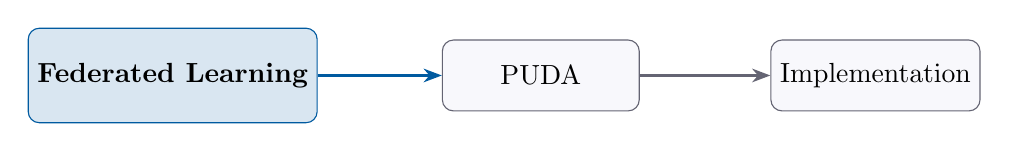
\begin{tikzpicture}[scale=0.85]
        \node[draw=primary,fill=primary!15,rounded corners,minimum width=3.5cm,minimum height=1.2cm,font=\bfseries] (fl) at (0,0) {Federated Learning};
        \node[draw=textmuted,fill=codebg,rounded corners,minimum width=2.5cm,minimum height=0.9cm] (puda) at (5.5,0) {PUDA};
        \node[draw=textmuted,fill=codebg,rounded corners,minimum width=2.5cm,minimum height=0.9cm] (tech) at (10.5,0) {Implementation};

        \draw[-{Stealth},thick,primary] (fl) -- (puda);
        \draw[-{Stealth},thick,textmuted] (puda) -- (tech);
    \end{tikzpicture}
    \end{center}

    \vspace{0.8cm}

    \begin{center}
        {\Large\textcolor{primary}{Why do we need secure aggregation?}}
    \end{center}

    \vspace{0.5cm}

    \begin{columns}[c]
        \begin{column}{0.45\textwidth}
            \centering
            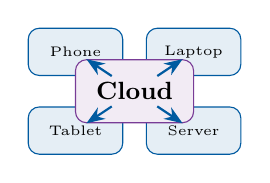
\begin{tikzpicture}[scale=0.5,
                device/.style={rectangle, rounded corners, draw=primary, fill=primary!10, minimum width=1.2cm, minimum height=0.6cm, font=\tiny}
            ]
                \node[device] (d1) at (-1.5,1.5) {Phone};
                \node[device] (d2) at (1.5,1.5) {Laptop};
                \node[device] (d3) at (-1.5,-0.5) {Tablet};
                \node[device] (d4) at (1.5,-0.5) {Server};
                \node[rectangle, rounded corners, draw=secondary, fill=secondary!10, minimum width=1.5cm, minimum height=0.8cm, font=\small\bfseries] (srv) at (0,0.5) {Cloud};

                \draw[-{Stealth},primary,thick] (d1) -- (srv);
                \draw[-{Stealth},primary,thick] (d2) -- (srv);
                \draw[-{Stealth},primary,thick] (d3) -- (srv);
                \draw[-{Stealth},primary,thick] (d4) -- (srv);
            \end{tikzpicture}
        \end{column}
        \begin{column}{0.45\textwidth}
            \small
            Data stays local, only \textbf{gradients} are shared.\\[0.3em]
            But gradients can \textcolor{danger}{leak information}!
        \end{column}
    \end{columns}
\end{frame}

\begin{frame}{What is Federated Learning?}
    \begin{columns}[T]
        \begin{column}{0.55\textwidth}
            \begin{block}{Definition}
                Machine learning approach where the model is trained across \textbf{decentralized devices} holding local data, without exchanging raw data.
            \end{block}

            \vspace{0.4em}
            \textbf{How it works:}
            \begin{itemize}
                \item Data remains on device (privacy by design)
                \item Each device computes local gradients
                \item Only gradients are sent to central server
                \item Server aggregates: $\nabla_{\text{global}} = \frac{1}{n}\sum_i \nabla_i$
                \item Updated model is sent back to devices
            \end{itemize}

            \vspace{0.4em}
            \textbf{The catch:}
            \begin{itemize}
                \item Gradients can leak training data
                \item Server sees individual contributions
            \end{itemize}
        \end{column}
        \begin{column}{0.42\textwidth}
            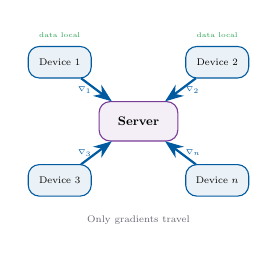
\begin{tikzpicture}[scale=0.5, transform shape,
                device/.style={rectangle, rounded corners, draw=primary, fill=primary!8, minimum width=1.6cm, minimum height=0.8cm, font=\scriptsize},
                server/.style={rectangle, rounded corners, draw=secondary, fill=secondary!8, minimum width=2cm, minimum height=1cm, font=\small\bfseries},
                arrow/.style={-{Stealth}, thick}
            ]
                \node[device] (d1) at (-2,2.5) {Device 1};
                \node[device] (d2) at (2,2.5) {Device 2};
                \node[device] (d3) at (-2,-0.5) {Device 3};
                \node[device] (d4) at (2,-0.5) {Device $n$};
                \node[server] (srv) at (0,1) {Server};

                \draw[arrow,primary] (d1) -- node[left,font=\tiny] {$\nabla_1$} (srv);
                \draw[arrow,primary] (d2) -- node[right,font=\tiny] {$\nabla_2$} (srv);
                \draw[arrow,primary] (d3) -- node[left,font=\tiny] {$\nabla_3$} (srv);
                \draw[arrow,primary] (d4) -- node[right,font=\tiny] {$\nabla_n$} (srv);

                \node[font=\tiny,text=success] at (-2,3.2) {data local};
                \node[font=\tiny,text=success] at (2,3.2) {data local};

                \node[font=\scriptsize,text=textmuted] at (0,-1.5) {Only gradients travel};
            \end{tikzpicture}

            \vspace{0.5em}
            \textbf{Applications:}
            \begin{itemize}
                \item Google Keyboard
                \item Apple Siri
                \item Medical research
                \item Banking fraud detection
            \end{itemize}
        \end{column}
    \end{columns}
\end{frame}

\begin{frame}{The Secure Aggregation Problem}
    \begin{alertblock}{Privacy Gap}
        Even without raw data, a \textbf{malicious server} can infer training data from gradients (gradient inversion attacks) and track individual contributions.
    \end{alertblock}

    \vspace{0.3em}

    \begin{columns}[T]
        \begin{column}{0.48\textwidth}
            \textbf{Existing approaches:}
            \begin{itemize}
                \item \textbf{Differential Privacy}
                    \begin{itemize}
                        \item[$+$] Provable guarantees
                        \item[$-$] Utility loss (noise added)
                    \end{itemize}
                \item \textbf{Secure MPC}
                    \begin{itemize}
                        \item[$+$] Perfect security
                        \item[$-$] High communication cost
                    \end{itemize}
                \item \textbf{Homomorphic Encryption}
                    \begin{itemize}
                        \item[$+$] Compute on ciphertexts
                        \item[$-$] Very slow in practice
                    \end{itemize}
            \end{itemize}
        \end{column}
        \begin{column}{0.48\textwidth}
            \begin{block}{What we need}
                \begin{enumerate}
                    \item \textbf{Privacy}: Individual values hidden
                    \item \textbf{Accuracy}: Exact result (no noise)
                    \item \textbf{Verifiability}: Detect tampering
                    \item \textbf{Efficiency}: Practical performance
                \end{enumerate}
            \end{block}

            \vspace{0.5em}
            \centering
            {\Large $\Downarrow$}\\[0.3em]
            {\Large\textbf{\textcolor{primary}{PUDA Protocol}}}
        \end{column}
    \end{columns}
\end{frame}

% ==============================================================================
% TRANSITION: PUDA PROTOCOL
% ==============================================================================
\begin{frame}{PUDA Protocol}
    \begin{center}
    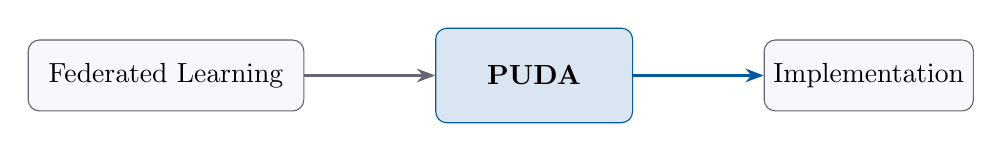
\begin{tikzpicture}[scale=0.85]
        \node[draw=textmuted,fill=codebg,rounded corners,minimum width=3.5cm,minimum height=0.9cm] (fl) at (0,0) {Federated Learning};
        \node[draw=primary,fill=primary!15,rounded corners,minimum width=2.5cm,minimum height=1.2cm,font=\bfseries] (puda) at (5.5,0) {PUDA};
        \node[draw=textmuted,fill=codebg,rounded corners,minimum width=2.5cm,minimum height=0.9cm] (tech) at (10.5,0) {Implementation};

        \draw[-{Stealth},thick,textmuted] (fl) -- (puda);
        \draw[-{Stealth},thick,primary] (puda) -- (tech);
    \end{tikzpicture}
    \end{center}

    \vspace{0.6cm}

    \begin{center}
        {\Large\textcolor{primary}{How does PUDA work?}}
    \end{center}

    \vspace{0.4cm}

    \textbf{PUDA} = \textbf{P}rivate \textbf{U}ser \textbf{D}ata \textbf{A}ggregation

    \vspace{0.3em}

    A cryptographic protocol that enables:
    \begin{itemize}
        \item Privacy-preserving aggregation using \textbf{mask cancellation}
        \item Public verifiability using \textbf{bilinear pairings}
        \item Exact results (no noise, no approximation)
    \end{itemize}
\end{frame}

\begin{frame}[fragile]{PUDA: Protocol Overview}
    \begin{center}
    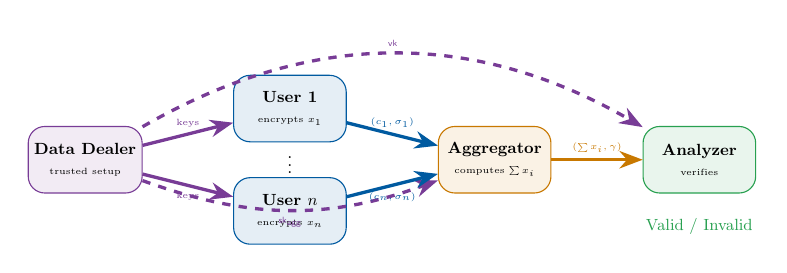
\begin{tikzpicture}[scale=0.65, transform shape,
        actor/.style={rectangle, rounded corners=6pt, draw=#1, fill=#1!10, minimum width=2.2cm, minimum height=1.3cm, font=\small, align=center},
        arrow/.style={-{Stealth}, line width=1.2pt}
    ]
        \node[actor=secondary] (dd) at (0,0) {\textbf{Data Dealer}\\{\tiny trusted setup}};
        \node[actor=primary] (u1) at (4,1) {\textbf{User 1}\\{\tiny encrypts $x_1$}};
        \node[actor=primary] (un) at (4,-1) {\textbf{User $n$}\\{\tiny encrypts $x_n$}};
        \node[actor=warning] (agg) at (8,0) {\textbf{Aggregator}\\{\tiny computes $\sum x_i$}};
        \node[actor=success] (ana) at (12,0) {\textbf{Analyzer}\\{\tiny verifies}};

        \draw[arrow,secondary] (dd) -- node[above,font=\tiny] {keys} (u1);
        \draw[arrow,secondary] (dd) -- node[below,font=\tiny] {keys} (un);
        \draw[arrow,secondary,dashed] (dd) to[bend right=20] node[below,font=\tiny] {$\mathsf{sk}_{\mathsf{agg}}$} (agg);
        \draw[arrow,secondary,dashed] (dd) to[bend left=30] node[above,font=\tiny] {$\mathsf{vk}$} (ana);

        \draw[arrow,primary] (u1) -- node[above,font=\tiny] {$(c_1,\sigma_1)$} (agg);
        \draw[arrow,primary] (un) -- node[below,font=\tiny] {$(c_n,\sigma_n)$} (agg);

        \draw[arrow,warning] (agg) -- node[above,font=\tiny] {$(\sum x_i, \gamma)$} (ana);

        \node[font=\small,text=success] at (12,-1.3) {Valid / Invalid};
        \node at (4,0) {$\vdots$};
    \end{tikzpicture}
    \end{center}

    \vspace{0.2em}

    \begin{columns}[T]
        \begin{column}{0.24\textwidth}
            \centering\small
            \textcolor{secondary}{\textbf{1. Setup}}\\
            Key generation\\
            {\tiny (once)}
        \end{column}
        \begin{column}{0.24\textwidth}
            \centering\small
            \textcolor{primary}{\textbf{2. EncTag}}\\
            Encrypt + tag\\
            {\tiny (per user)}
        \end{column}
        \begin{column}{0.24\textwidth}
            \centering\small
            \textcolor{warning}{\textbf{3. Aggregate}}\\
            Compute sum\\
            {\tiny (mask cancellation)}
        \end{column}
        \begin{column}{0.24\textwidth}
            \centering\small
            \textcolor{success}{\textbf{4. Verify}}\\
            Check integrity\\
            {\tiny (pairings)}
        \end{column}
    \end{columns}
\end{frame}

\begin{frame}{Threat Model}
    \begin{columns}[T]
        \begin{column}{0.48\textwidth}
            \begin{block}{Adversarial Model}
                \begin{itemize}
                    \item \textbf{Data Dealer}: Trusted (runs once)
                    \item \textbf{Users}: Honest (follow protocol)
                    \item \textbf{Aggregator}: \textcolor{danger}{Semi-honest}
                    \item \textbf{Analyzer}: Public verifier
                \end{itemize}
            \end{block}

            \vspace{0.3em}

            \begin{block}{Semi-honest Adversary $\Adv$}
                The aggregator:
                \begin{itemize}
                    \item Executes protocol correctly
                    \item Tries to learn individual $x_i$ from the transcript $\{(c_i, \sigma_i)\}_{i \in [n]}$
                \end{itemize}
            \end{block}
        \end{column}
        \begin{column}{0.48\textwidth}
            \begin{block}{Security Properties}
                \textbf{Privacy:}
                \begin{itemize}
                    \item $\Adv$ cannot distinguish $(x_i)$ from $(x'_i)$ with same aggregate
                    \item Reduces to CDH in $\G_1$
                \end{itemize}

                \vspace{0.3em}
                \textbf{Verifiability:}
                \begin{itemize}
                    \item $\Adv$ cannot forge valid $(\tilde{X}, \tilde{\gamma})$ with $\tilde{X} \neq \sum x_i$
                    \item Reduces to co-CDH
                \end{itemize}

                \vspace{0.3em}
                \textbf{Correctness:}
                \begin{itemize}
                    \item Honest execution yields $X_k = \sum_{i} x_{i,k}$
                \end{itemize}
            \end{block}
        \end{column}
    \end{columns}
\end{frame}

% ==============================================================================
% TRANSITION: TECHNICAL CHOICES
% ==============================================================================
\begin{frame}[fragile]{Technical Choices}
    \begin{center}
    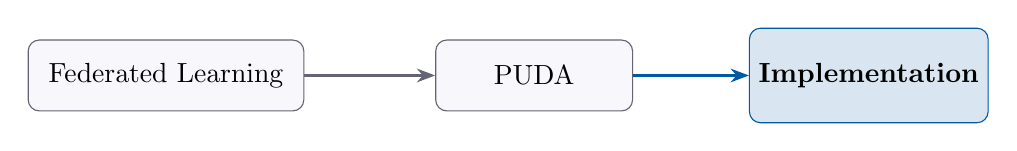
\begin{tikzpicture}[scale=0.85]
        \node[draw=textmuted,fill=codebg,rounded corners,minimum width=3.5cm,minimum height=0.9cm] (fl) at (0,0) {Federated Learning};
        \node[draw=textmuted,fill=codebg,rounded corners,minimum width=2.5cm,minimum height=0.9cm] (puda) at (5.5,0) {PUDA};
        \node[draw=primary,fill=primary!15,rounded corners,minimum width=2.8cm,minimum height=1.2cm,font=\bfseries] (tech) at (10.5,0) {Implementation};

        \draw[-{Stealth},thick,textmuted] (fl) -- (puda);
        \draw[-{Stealth},thick,primary] (puda) -- (tech);
    \end{tikzpicture}
    \end{center}

    \vspace{0.5cm}

    \begin{center}
    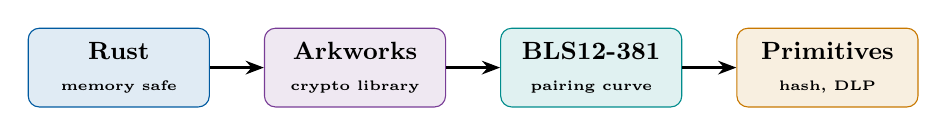
\begin{tikzpicture}[scale=0.75,
        box/.style={rectangle, rounded corners, draw=#1, fill=#1!12, minimum width=2.3cm, minimum height=1cm, font=\small\bfseries, align=center}
    ]
        \node[box=primary] (rust) at (0,0) {Rust\\{\tiny memory safe}};
        \node[box=secondary] (ark) at (4,0) {Arkworks\\{\tiny crypto library}};
        \node[box=accent] (bls) at (8,0) {BLS12-381\\{\tiny pairing curve}};
        \node[box=warning] (hash) at (12,0) {Primitives\\{\tiny hash, DLP}};

        \draw[-{Stealth},thick] (rust) -- (ark);
        \draw[-{Stealth},thick] (ark) -- (bls);
        \draw[-{Stealth},thick] (bls) -- (hash);
    \end{tikzpicture}
    \end{center}
\end{frame}

\begin{frame}{Rust and Arkworks}
    \begin{columns}[T]
        \begin{column}{0.48\textwidth}
            \begin{block}{Language: Rust}
                \begin{itemize}
                    \item Memory safety without garbage collector
                    \item Zero-cost abstractions
                    \item Strong type system
                    \item No undefined behavior
                \end{itemize}
            \end{block}

            \vspace{0.4em}
            \textbf{Why it matters for crypto:}
            \begin{itemize}
                \item Constant-time operations possible
                \item Memory zeroization (secrets don't leak)
                \item No implicit copies of sensitive data
                \item Compiler catches many bugs
            \end{itemize}
        \end{column}
        \begin{column}{0.48\textwidth}
            \begin{block}{Library: Arkworks}
                \textbf{ark-bls12-381:}
                \begin{itemize}
                    \item Pairing-friendly elliptic curve
                    \item 128-bit security level
                    \item Optimized implementation
                \end{itemize}

                \vspace{0.3em}
                \textbf{ark-ec, ark-ff:}
                \begin{itemize}
                    \item Elliptic curve arithmetic
                    \item Finite field operations
                    \item Serialization utilities
                \end{itemize}
            \end{block}

            \vspace{0.3em}
            \begin{exampleblock}{Ecosystem}
                Same libraries used by:\\Zcash, Aleo, Mina Protocol
            \end{exampleblock}
        \end{column}
    \end{columns}
\end{frame}

\begin{frame}{BLS12-381: Algebraic Structure}
    \begin{columns}[T]
        \begin{column}{0.52\textwidth}
            \begin{block}{Three Groups}
                Cyclic groups of prime order $r \approx 2^{255}$:
                \begin{align*}
                    \G_1 &\subset E(\F_p) & \text{(48 bytes compressed)}\\
                    \G_2 &\subset E'(\F_{p^2}) & \text{(96 bytes compressed)}\\
                    \G_T &\subset \F_{p^{12}}^* & \text{(target group)}
                \end{align*}
            \end{block}

            \vspace{0.3em}
            \textbf{Bilinear Pairing:}
            \[
            e: \G_1 \times \G_2 \to \G_T
            \]

            \textbf{Key property (bilinearity):}
            \[
            \boxed{e([a]P, [b]Q) = e(P, Q)^{ab}}
            \]
        \end{column}
        \begin{column}{0.45\textwidth}
            \begin{block}{Why pairings?}
                Enable verification without secrets:
                \[
                e(\gamma, P_2) \stackrel{?}{=} \prod_k e(V_k, \mathsf{vk}_k)
                \]

                \begin{itemize}
                    \item Check $\G_1$-$\G_2$ relationships
                    \item Without revealing scalar values
                    \item Anyone can verify (public)
                \end{itemize}
            \end{block}

            \vspace{0.3em}
            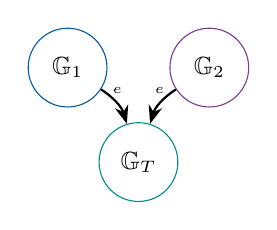
\begin{tikzpicture}[scale=0.6]
                \node[draw=primary,circle,minimum size=1cm,font=\small] (g1) at (0,0) {$\G_1$};
                \node[draw=secondary,circle,minimum size=1cm,font=\small] (g2) at (3,0) {$\G_2$};
                \node[draw=accent,circle,minimum size=1cm,font=\small] (gt) at (1.5,-2) {$\G_T$};

                \draw[-{Stealth},thick] (g1) to[bend left=20] node[above,font=\tiny] {$e$} (gt);
                \draw[-{Stealth},thick] (g2) to[bend right=20] node[above,font=\tiny] {$e$} (gt);
            \end{tikzpicture}
        \end{column}
    \end{columns}
\end{frame}

\begin{frame}{Hash-to-$\G_1$: Mapping Strings to Curve Points}
    \begin{columns}[T]
        \begin{column}{0.48\textwidth}
            \begin{block}{The Problem}
                Need function $\Hash: \{0,1\}^* \to \G_1$

                \vspace{0.2em}
                \textbf{Used for:} computing $\Hash(\tau \| k)$ in encryption
            \end{block}

            \vspace{0.3em}
            \textbf{Challenge:}
            \begin{itemize}
                \item Curve equation: $y^2 = x^3 + 4$
                \item Not every $x \in \F_p$ yields valid $y$
                \item Only $\sim 50\%$ of $x$ values work
            \end{itemize}

            \vspace{0.3em}
            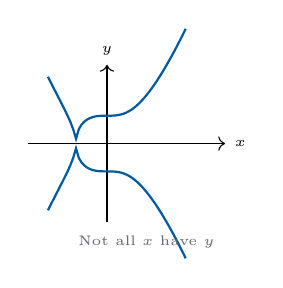
\begin{tikzpicture}[scale=0.5]
                \draw[->] (-2,0) -- (3,0) node[right,font=\tiny] {$x$};
                \draw[->] (0,-2) -- (0,2) node[above,font=\tiny] {$y$};
                \draw[domain=-1.5:2,samples=50,primary,thick] plot (\x, {sqrt(abs(\x*\x*\x + 0.5))});
                \draw[domain=-1.5:2,samples=50,primary,thick] plot (\x, {-sqrt(abs(\x*\x*\x + 0.5))});
                \node[font=\tiny,text=textmuted] at (1,-2.5) {Not all $x$ have $y$};
            \end{tikzpicture}
        \end{column}
        \begin{column}{0.48\textwidth}
            \begin{block}{Solution: Try-and-Increment}
                \begin{enumerate}
                    \item Hash input with counter
                    \item Interpret as $x$-coordinate
                    \item Check if $y^2 = x^3 + 4$ is square
                    \item If yes: compute $y$, return point
                    \item If no: increment counter, retry
                \end{enumerate}
            \end{block}

            \vspace{0.3em}
            \textbf{Important details:}
            \begin{itemize}
                \item Uses SHA-512 for hashing
                \item Legendre symbol to check quadratic residue
                \item Cofactor multiplication for subgroup
                \item Expected iterations: $\sim 2$
            \end{itemize}
        \end{column}
    \end{columns}
\end{frame}

\begin{frame}[fragile]{Hash-to-$\G_1$: Implementation}
    \textbf{Key insight:} We hash, check if valid curve point exists, multiply by cofactor to land in $\G_1$.

    \vspace{0.3em}
\begin{lstlisting}[style=rust]
pub fn map_to_group(message: &str) -> G1 {
    let mut counter = 0u64;
    loop {
        // 1. Hash message with counter to get x-coordinate candidate
        let input_str = format!("{:0width$b}{}", counter, message, width = max_iterations);
        let (x, sign_selector) = h_prime(input_str.as_bytes());  // Uses SHA-512

        // 2. Compute f(x) = x^3 + ax + b (curve equation)
        let f_x = x.pow([3]) + coeff_a * x + coeff_b;

        // 3. Check if f(x) is a quadratic residue (Legendre symbol)
        if f_x.legendre().is_qr() {
            let root = f_x.sqrt().unwrap();         // Compute y = sqrt(f(x))
            let point = G1Affine::new_unchecked(x, root);

            // 4. Multiply by cofactor to ensure point is in G1 subgroup
            let final_point = point.into_group().mul_bigint(cofactor_big);
            if !final_point.is_zero() { return final_point; }
        }
        counter += 1;  // Try next candidate
    }
}
\end{lstlisting}
\end{frame}

\begin{frame}[fragile]{DLP Table: Discrete Log Recovery}
    \textbf{Problem:} After mask cancellation, we have $V = [X]P_1$. How to recover integer $X$?

    \vspace{0.3em}

    \begin{columns}[T]
        \begin{column}{0.45\textwidth}
            \begin{block}{Solution: Precomputed Table}
                Build lookup table at startup:
                \[
                T = \{[i]P_1 \mapsto i\}_{i=0}^{65535}
                \]

                \textbf{Query:} serialize $V$, lookup in HashMap

                \textbf{Complexity:} $O(1)$ per lookup
            \end{block}

            \vspace{0.2em}
            \begin{alertblock}{Constraint}
                $n \times \max(x_i) < 65536$

                With $n=100$: $\max \leq 655$
            \end{alertblock}
        \end{column}
        \begin{column}{0.52\textwidth}
\begin{lstlisting}[style=rust]
const DLP_TABLE_SIZE: u64 = 65536;

fn init_dlp_lookup_table() -> HashMap<Vec<u8>, u64> {
    let g1_gen = G1::generator();
    let mut table = HashMap::new();
    let mut current = G1::zero();  // Start at identity

    for i in 0..DLP_TABLE_SIZE {
        let mut bytes = Vec::new();
        current.serialize_compressed(&mut bytes);
        table.insert(bytes, i);  // Map point -> scalar
        current += g1_gen;       // Next: (i+1)*G
    }
    table
}

pub fn find_discrete_log(target: G1) -> u64 {
    let mut bytes = Vec::new();
    target.serialize_compressed(&mut bytes);
    *DLP_TABLE.get(&bytes).unwrap()  // O(1) lookup
}
\end{lstlisting}
        \end{column}
    \end{columns}
\end{frame}

% ==============================================================================
% TRANSITION: THE FOUR PHASES
% ==============================================================================
\begin{frame}[fragile]{The Four Phases}
    \begin{center}
    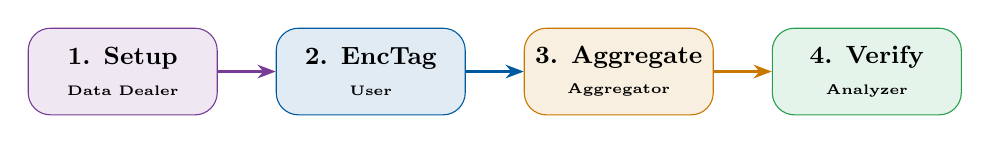
\begin{tikzpicture}[scale=0.75,
        phase/.style={rectangle, rounded corners=8pt, draw=#1, fill=#1!12, minimum width=2.4cm, minimum height=1.1cm, font=\small\bfseries, align=center}
    ]
        \node[phase=secondary] (setup) at (0,0) {1. Setup\\{\tiny Data Dealer}};
        \node[phase=primary] (enc) at (4.2,0) {2. EncTag\\{\tiny User}};
        \node[phase=warning] (agg) at (8.4,0) {3. Aggregate\\{\tiny Aggregator}};
        \node[phase=success] (ver) at (12.6,0) {4. Verify\\{\tiny Analyzer}};

        \draw[-{Stealth},thick,secondary] (setup) -- (enc);
        \draw[-{Stealth},thick,primary] (enc) -- (agg);
        \draw[-{Stealth},thick,warning] (agg) -- (ver);
    \end{tikzpicture}
    \end{center}

    \vspace{0.6cm}

    \begin{columns}[T]
        \begin{column}{0.24\textwidth}
            \centering
            \textcolor{secondary}{Keys}\\
            $\downarrow$\\
            {\small All actors}\\[0.5em]
            {\tiny $\mathsf{sk}_{\mathsf{agg}} = -\sum \mathsf{ek}_i$}
        \end{column}
        \begin{column}{0.24\textwidth}
            \centering
            \textcolor{primary}{$(c_i, \sigma_i)$}\\
            $\downarrow$\\
            {\small Aggregator}\\[0.5em]
            {\tiny masked ciphertexts}
        \end{column}
        \begin{column}{0.24\textwidth}
            \centering
            \textcolor{warning}{$(\sum x_i, \gamma)$}\\
            $\downarrow$\\
            {\small Analyzer}\\[0.5em]
            {\tiny masks cancelled}
        \end{column}
        \begin{column}{0.24\textwidth}
            \centering
            \textcolor{success}{Valid/Invalid}\\
            $\downarrow$\\
            {\small Result}\\[0.5em]
            {\tiny pairing check}
        \end{column}
    \end{columns}
\end{frame}

% --- PHASE 1: SETUP ---
\begin{frame}{Phase 1: Setup (Data Dealer)}
    \begin{columns}[T]
        \begin{column}{0.48\textwidth}
            \begin{alertblock}{Input}
                \begin{itemize}
                    \item $n$: number of users
                    \item $\kappa$: vector dimension
                \end{itemize}
            \end{alertblock}

            \begin{exampleblock}{Output}
                \begin{itemize}
                    \item $\mathsf{pp} = (P_1, P_2)$: generators
                    \item $\{(\mathsf{ek}_i, \mathsf{tk}_i)\}$: user keys
                    \item $\mathsf{sk}_{\mathsf{agg}}$: aggregator key
                    \item $\mathsf{vk}$: verification key
                \end{itemize}
            \end{exampleblock}
        \end{column}
        \begin{column}{0.48\textwidth}
            \begin{block}{Algorithm}
                \begin{enumerate}
                    \item Sample generators $P_1, P_2$
                    \item Sample tag coefficients $\mathbf{a} \xleftarrow{\$} \F_r^\kappa$
                    \item For each user $i$:
                    \begin{itemize}
                        \item $\mathsf{ek}_i \xleftarrow{\$} \F_r$ (encryption key)
                        \item $b_i \xleftarrow{\$} \F_r$ (tag component)
                    \end{itemize}
                    \item Compute $\mathsf{sk}_{\mathsf{agg}} = -\sum_{i} \mathsf{ek}_i$
                    \item Compute $\mathsf{vk}_a, \mathsf{vk}_b$ in $\G_2$
                \end{enumerate}
            \end{block}

            \textbf{Key constraint:}
            \[
            \boxed{\mathsf{sk}_{\mathsf{agg}} = -\sum_{i=1}^n \mathsf{ek}_i}
            \]
        \end{column}
    \end{columns}
\end{frame}

\begin{frame}[fragile]{Phase 1: Setup -- Code}
    \textbf{Key insight:} We accumulate all $\mathsf{ek}_i$ into \texttt{ak}, then negate it for the aggregator key.

    \vspace{0.3em}
\begin{lstlisting}[style=rust]
pub fn setup(num_users: usize, rng: &mut StdRng, kappa: usize)
    -> (PublicParams, Vec<UserSecretKey>, AggregatorSecretKey, DataDealerVK)
{
    let p_1 = G1::generator();
    let p_2 = G2::generator();

    // Tag coefficients: a = (a_1, ..., a_kappa) sampled uniformly
    let a: Vec<ScalarField> = (0..kappa).map(|_| ScalarField::rand(rng)).collect();
    let vk_a: Vec<G2> = a.iter().map(|a_val| p_2 * a_val).collect();  // vk_a[k] = a[k] * P2

    let mut ak: ScalarField = ScalarField::zero();  // Will accumulate sum of ek_i

    for i in 0..num_users {
        let ek_i = ScalarField::rand(rng);  // Random encryption key
        ak += ek_i;                          // Accumulate for aggregator key
        let b_i = ScalarField::rand(rng);    // Random tag component
        vk_b[i] = p_2 * b_i;                 // vk_b[i] = b_i * P2
        user_keys.push(UserSecretKey { id: i, ek: ek_i, tk: (a.clone(), b_i) });
    }

    let aggregator_key = AggregatorSecretKey { ska: -ak };  // NEGATION enables mask cancellation
    // ...
}
\end{lstlisting}
\end{frame}

% --- PHASE 2: ENCTAG ---
\begin{frame}{Phase 2: EncTag (User)}
    \begin{columns}[T]
        \begin{column}{0.48\textwidth}
            \begin{alertblock}{Input}
                \begin{itemize}
                    \item $\mathbf{x}_i = (x_{i,1}, \ldots, x_{i,\kappa})$: data
                    \item $\tau$: session identifier
                    \item $(\mathsf{ek}_i, \mathsf{tk}_i)$: user keys
                \end{itemize}
            \end{alertblock}

            \begin{exampleblock}{Output}
                \begin{itemize}
                    \item $\mathbf{c}_i \in \G_1^\kappa$: ciphertexts
                    \item $\sigma_i \in \G_1$: authentication tag
                \end{itemize}
            \end{exampleblock}

            \vspace{0.3em}
            \textbf{Privacy:} The mask $\mathsf{ek}_i \cdot \Hash(\tau\|k)$ hides $x_{i,k}$ under CDH assumption.
        \end{column}
        \begin{column}{0.48\textwidth}
            \begin{block}{Formulas}
                \textbf{Ciphertext} (for each $k$):
                \[
                c_{i,k} = \underbrace{[x_{i,k}] P_1}_{\text{data}} + \underbrace{[\mathsf{ek}_i] \cdot \Hash(\tau \| k)}_{\text{mask}}
                \]

                \vspace{0.3em}
                \textbf{Tag}:
                \[
                \sigma_i = \underbrace{[b_i] \cdot \Hash(\tau)}_{\text{user binding}} + \underbrace{\sum_{k} [a_k x_{i,k}] P_1}_{\text{data commitment}}
                \]
            \end{block}

            \vspace{0.2em}
            The tag commits to all values while binding to user identity via $b_i$.
        \end{column}
    \end{columns}
\end{frame}

\begin{frame}[fragile]{Phase 2: EncTag -- Code}
    \textbf{Key insight:} Each ciphertext $c[k]$ combines encoded data with a mask. The tag commits to all data.

    \vspace{0.3em}
\begin{lstlisting}[style=rust]
pub fn enc_tag(uk: &UserSecretKey, x_i: Vec<u64>, tau: u64,
               kappa: usize, pp: &PublicParams) -> CiphertextAndTag
{
    // 1. Compute ciphertexts: c[k] = x[k]*P1 + ek*H(tau||k)
    let mut c: Vec<G1> = vec![G1::zero(); kappa];
    for k in 0..kappa {
        let h = map_to_group(&format!("{}{}", tau, k));  // H(tau||k)
        c[k] = pp.p_1 * ScalarField::from(x_i[k])        // Data: x[k] * P1
             + h * uk.ek;                                 // Mask: ek * H(tau||k)
    }

    // 2. Compute tag: sigma = b*H(tau) + Sum(a[k] * x[k] * P1)
    let h_tau = map_to_group(&tau.to_string());
    let mut sigma = h_tau * uk.tk.1;  // User binding: b_i * H(tau)

    for (k, x_val) in x_i.iter().enumerate() {
        let a_k = uk.tk.0[k];
        sigma += pp.p_1 * (ScalarField::from(*x_val) * a_k);  // Data commitment
    }

    CiphertextAndTag { c, sigma }
}
\end{lstlisting}
\end{frame}

% --- PHASE 3: AGGREGATE ---
\begin{frame}{Phase 3: Aggregate (Aggregator)}
    \begin{columns}[T]
        \begin{column}{0.48\textwidth}
            \begin{alertblock}{Input}
                \begin{itemize}
                    \item $\{(\mathbf{c}_i, \sigma_i)\}_{i \in [n]}$: all ciphertexts
                    \item $\mathsf{sk}_{\mathsf{agg}}$: aggregator key
                    \item $\tau$: session identifier
                \end{itemize}
            \end{alertblock}

            \begin{exampleblock}{Output}
                \begin{itemize}
                    \item $\mathbf{X}$ where $X_k = \sum_i x_{i,k}$
                    \item $\gamma = \sum_i \sigma_i$
                \end{itemize}
            \end{exampleblock}

            \vspace{0.2em}
            \textbf{Privacy:} Aggregator learns $\sum x_i$ but \textbf{not} individual $x_i$ values!
        \end{column}
        \begin{column}{0.48\textwidth}
            \begin{block}{Mask Cancellation}
                For each $k$:
                \begin{align*}
                    V_k &= \sum_{i} c_{i,k} + [\mathsf{sk}_{\mathsf{agg}}] \cdot \Hash(\tau \| k)\\[0.3em]
                    &= \sum_i [x_{i,k}]P_1 + \underbrace{[\sum_i \mathsf{ek}_i + \mathsf{sk}_{\mathsf{agg}}]}_{= 0} \cdot \Hash\\[0.3em]
                    &= [X_k] P_1
                \end{align*}
            \end{block}

            Then: $X_k \gets \mathsf{DLP\_lookup}(V_k)$
        \end{column}
    \end{columns}
\end{frame}

\begin{frame}[fragile]{Phase 3: Aggregate -- Code}
    \textbf{Key insight:} Adding $\mathsf{sk}_{\mathsf{agg}} \cdot H$ cancels all the $\mathsf{ek}_i \cdot H$ masks, revealing $[X_k]P_1$.

    \vspace{0.3em}
\begin{lstlisting}[style=rust]
pub fn aggregate(agg_sk: &AggregatorSecretKey, inputs: &[CiphertextAndTag],
                 tau: u64, kappa: usize, _pp: &PublicParams) -> (Vec<u64>, G1)
{
    let mut x: Vec<u64> = Vec::new();

    for k in 0..kappa {
        let h = map_to_group(&format!("{}{}", tau, k));  // H(tau||k)

        // Sum all ciphertexts for dimension k
        let mut v = G1::zero();
        for ct in inputs {
            v += ct.c[k];  // v = sum of c_i[k]
        }

        v += h * agg_sk.ska;  // ADD aggregator's mask: CANCELS all user masks!

        x.push(find_discrete_log(v));  // Recover X_k from [X_k]P1
    }

    // Combine all tags
    let mut gamma = G1::zero();
    for ct in inputs { gamma += ct.sigma; }

    (x, gamma)
}
\end{lstlisting}
\end{frame}

% --- PHASE 4: VERIFY ---
\begin{frame}{Phase 4: Verify (Analyzer)}
    \begin{columns}[T]
        \begin{column}{0.48\textwidth}
            \begin{alertblock}{Input}
                \begin{itemize}
                    \item $(X_1, \ldots, X_\kappa)$: claimed aggregate
                    \item $\gamma \in \G_1$: combined tag
                    \item $\mathsf{vk} = (\mathsf{vk}_a, \mathsf{vk}_b)$
                    \item $\tau$: session identifier
                \end{itemize}
            \end{alertblock}

            \begin{exampleblock}{Output}
                \begin{itemize}
                    \item $\mathsf{accept}$: result is correct
                    \item $\mathsf{reject}$: tampering detected
                \end{itemize}
            \end{exampleblock}

            \vspace{0.2em}
            \textbf{Public verification:} No secrets needed!
        \end{column}
        \begin{column}{0.48\textwidth}
            \begin{block}{Pairing Equation}
                {\small
                \[
                e(\gamma, P_2) \stackrel{?}{=} \prod_{k} e([X_k]P_1, \mathsf{vk}_{a,k}) \cdot \prod_{i} e(H_\tau, \mathsf{vk}_{b,i})
                \]}
            \end{block}

            \vspace{0.2em}
            \textbf{Why it works:}
            \begin{itemize}
                \item Left side: pairing of combined tag
                \item Right side: reconstruction from $X_k$ and verification keys
                \item By bilinearity, equal iff consistent
            \end{itemize}
        \end{column}
    \end{columns}
\end{frame}

\begin{frame}[fragile]{Phase 4: Verify -- Code}
    \textbf{Key insight:} We compute both sides of the pairing equation and compare. If equal, the aggregation is correct.

    \vspace{0.3em}
\begin{lstlisting}[style=rust]
pub fn verify(data_vk: &DataDealerVK, gamma: G1, x_tau: Vec<u64>,
              tau: u64, kappa: usize, pp: &PublicParams) -> bool
{
    // LEFT SIDE: e(gamma, P2)
    let lhs = Bls12_381::pairing(gamma, pp.p_2).0;

    // RIGHT SIDE: product of pairings
    let mut rhs = TargetField::one();

    // Part 1: for each dimension k, compute e(X_k * P1, vk_a[k])
    for k in 0..kappa {
        rhs *= Bls12_381::pairing(
            pp.p_1 * ScalarField::from(x_tau[k]),  // X_k * P1
            data_vk.vk_a[k]                         // a_k * P2
        ).0;
    }

    // Part 2: for each user i, compute e(H(tau), vk_b[i])
    let h_tau = map_to_group(&tau.to_string());
    for i in 0..data_vk.vk_b.len() {
        rhs *= Bls12_381::pairing(h_tau, data_vk.vk_b[i]).0;
    }

    lhs == rhs  // True if aggregation is correct
}
\end{lstlisting}
\end{frame}

% ==============================================================================
% TRANSITION: PERFORMANCE ANALYSIS
% ==============================================================================
\begin{frame}{Performance Analysis}
    \begin{center}
    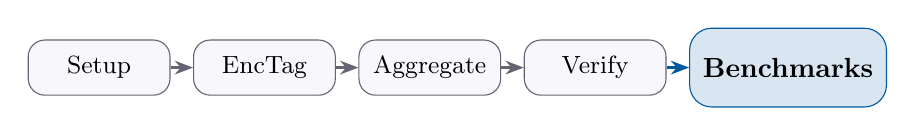
\begin{tikzpicture}[scale=0.7,
        phase/.style={rectangle, rounded corners=6pt, draw=textmuted, fill=codebg, minimum width=1.8cm, minimum height=0.7cm, font=\small}
    ]
        \node[phase] (setup) at (0,0) {Setup};
        \node[phase] (enc) at (3,0) {EncTag};
        \node[phase] (agg) at (6,0) {Aggregate};
        \node[phase] (ver) at (9,0) {Verify};
        \node[rectangle, rounded corners=8pt, draw=primary, fill=primary!15, minimum width=2.5cm, minimum height=1cm, font=\bfseries] (bench) at (12.5,0) {Benchmarks};

        \draw[-{Stealth},thick,textmuted] (setup) -- (enc);
        \draw[-{Stealth},thick,textmuted] (enc) -- (agg);
        \draw[-{Stealth},thick,textmuted] (agg) -- (ver);
        \draw[-{Stealth},thick,primary] (ver) -- (bench);
    \end{tikzpicture}
    \end{center}

    \vspace{0.8cm}

    \begin{center}
        {\Large\textcolor{primary}{Real measurements on my machine}}\\[0.5em]
        {\small Configuration: 5 trials average, $\max(x_i) = 650$, single-threaded}
    \end{center}
\end{frame}

\begin{frame}{Benchmark Results}
    \begin{columns}[T]
        \begin{column}{0.45\textwidth}
            \begin{center}
            \small
            \begin{tabular}{lcccc}
                \toprule
                \textbf{($n$, $\kappa$)} & \textbf{Setup} & \textbf{Enc} & \textbf{Agg} & \textbf{Ver} \\
                \midrule
                25, 25 & 55 & 641 & 173 & 125 \\
                50, 50 & 110 & 3422 & 294 & 311 \\
                75, 75 & 336 & 12000 & 495 & 857 \\
                100, 100 & 368 & 19189 & 734 & 878 \\
                \bottomrule
            \end{tabular}
            \end{center}
            {\tiny All times in milliseconds. Encryption is total for all $n$ users.}

            \vspace{0.5em}
            \textbf{Key finding:} Encryption takes \textbf{90\%+} of total time at scale. But it's parallelizable across users!
        \end{column}
        \begin{column}{0.52\textwidth}
            \centering
            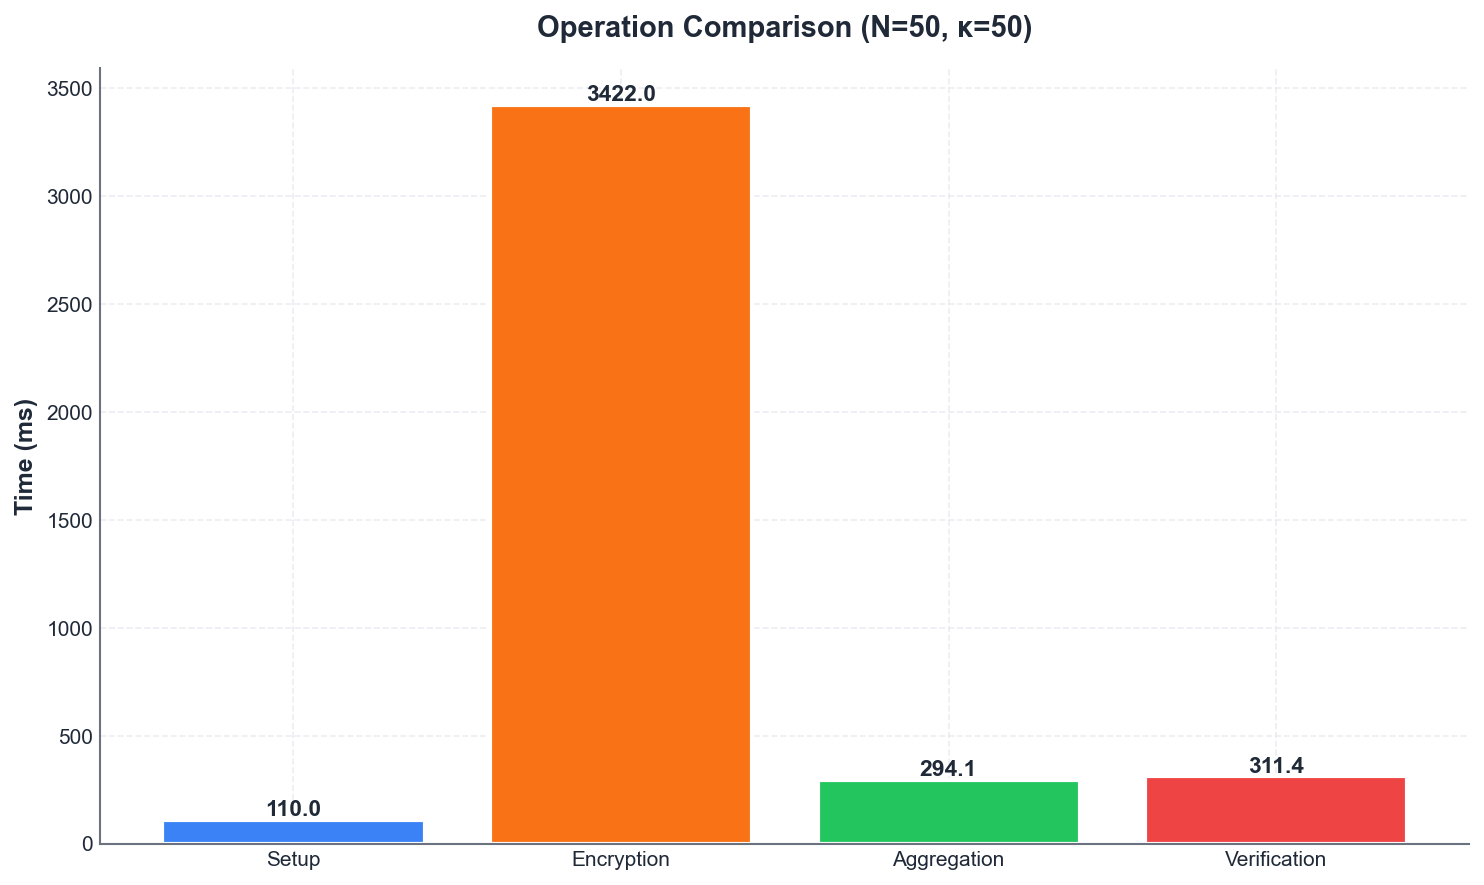
\includegraphics[width=\textwidth]{graph_bar_comparison.png}
        \end{column}
    \end{columns}
\end{frame}

\begin{frame}{Scaling with Users and Dimensions}
    \begin{columns}[T]
        \begin{column}{0.48\textwidth}
            \centering
            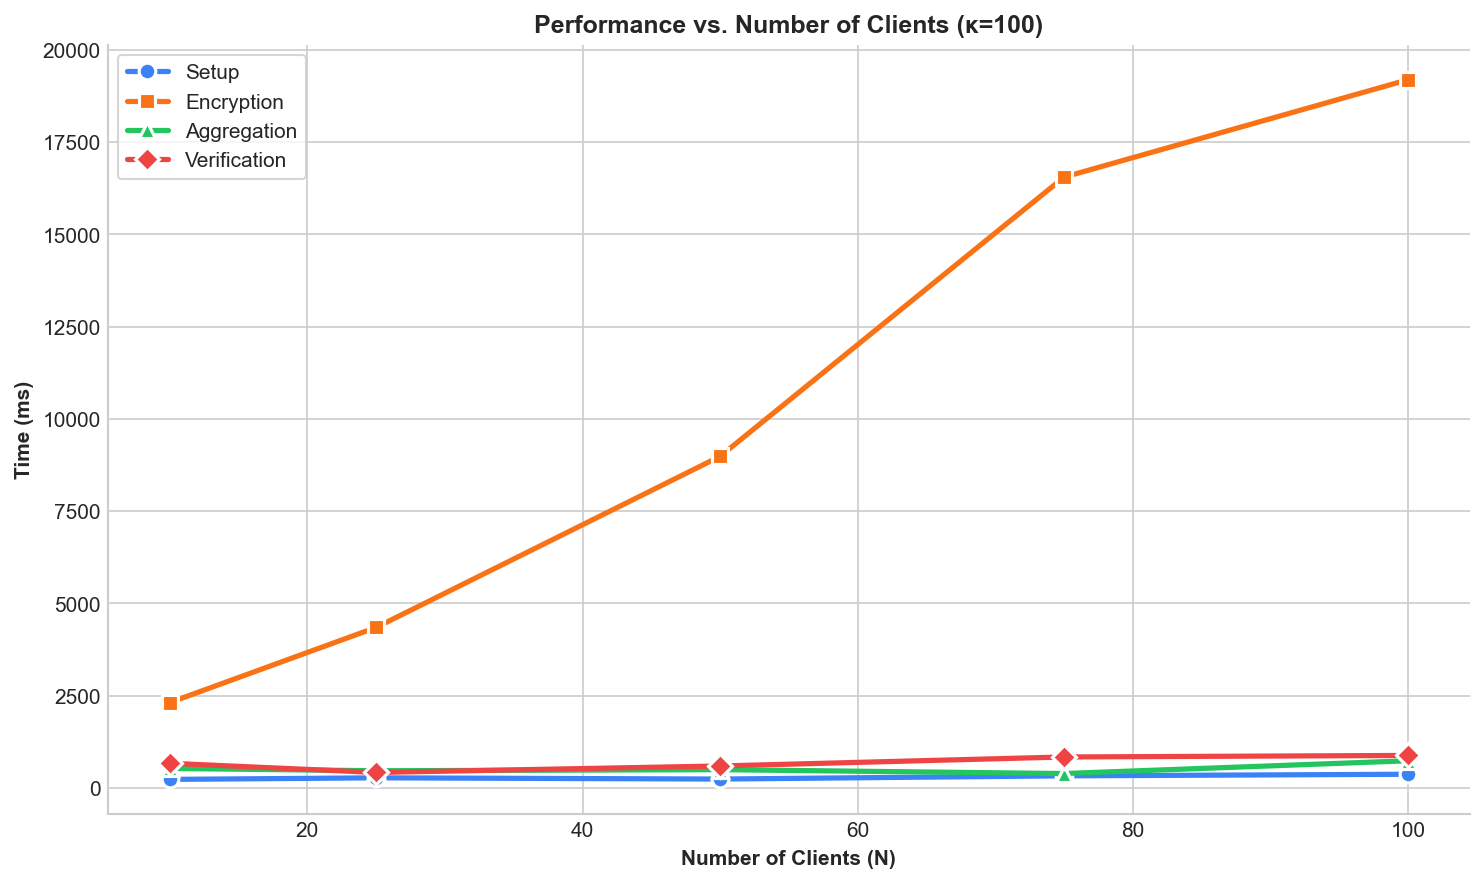
\includegraphics[width=0.98\textwidth]{graph_impact_users.png}
        \end{column}
        \begin{column}{0.48\textwidth}
            \centering
            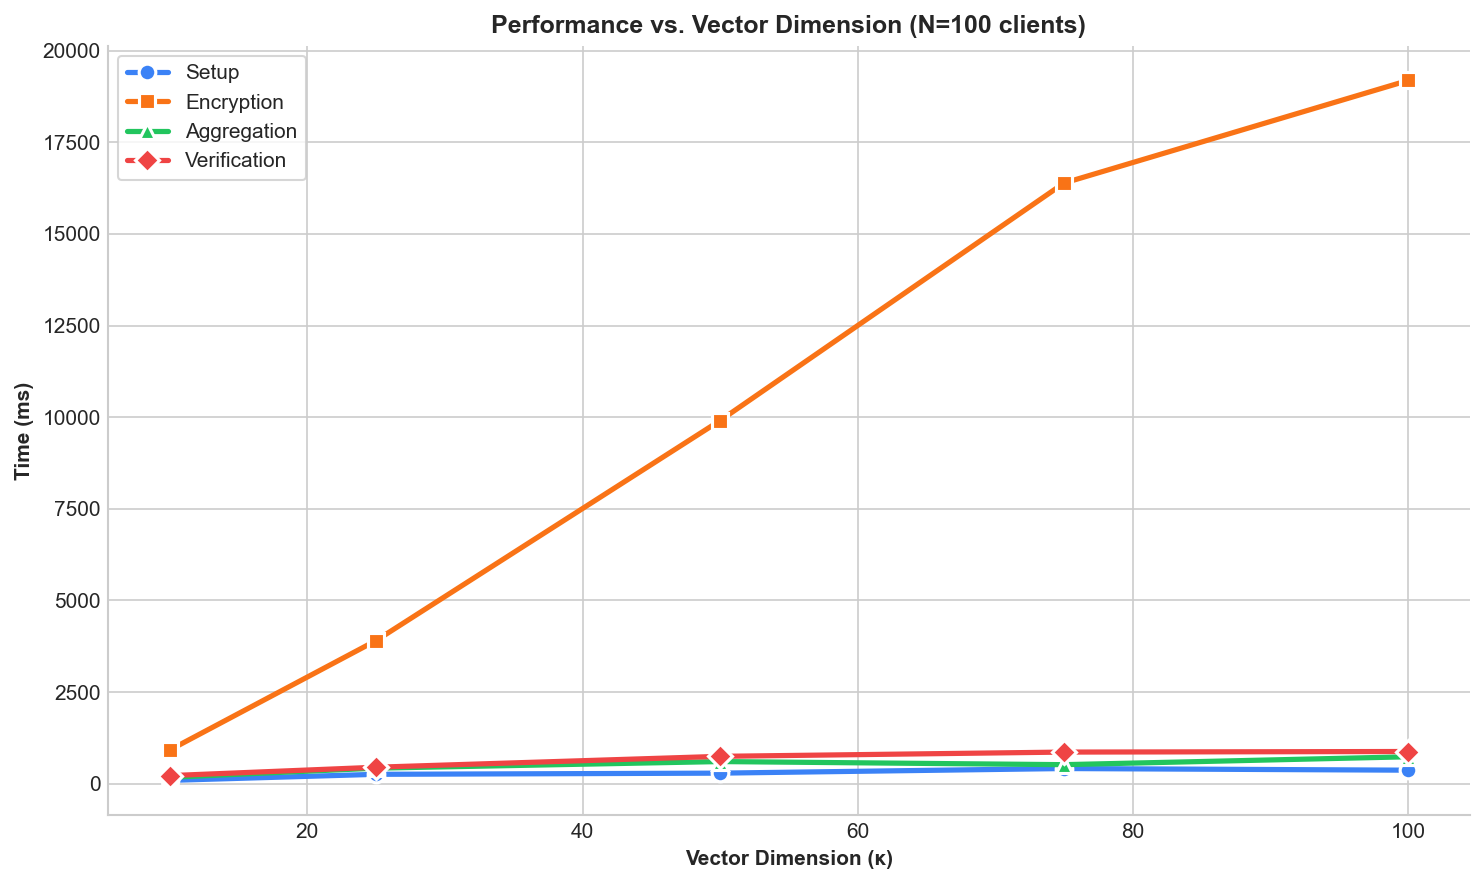
\includegraphics[width=0.98\textwidth]{graph_impact_kappa.png}
        \end{column}
    \end{columns}

    \vspace{0.3em}

    \begin{columns}[T]
        \begin{column}{0.48\textwidth}
            \textbf{Varying $n$ (users):}
            \begin{itemize}
                \item Encryption scales linearly ($n$ users)
                \item Aggregation nearly constant
                \item Verification linear in $n$
            \end{itemize}
        \end{column}
        \begin{column}{0.48\textwidth}
            \textbf{Varying $\kappa$ (dimensions):}
            \begin{itemize}
                \item All phases scale with $\kappa$
                \item Encryption per user: $O(\kappa)$
                \item Hash-to-curve dominates cost
            \end{itemize}
        \end{column}
    \end{columns}
\end{frame}

\begin{frame}{Scalability Analysis}
    \begin{center}
        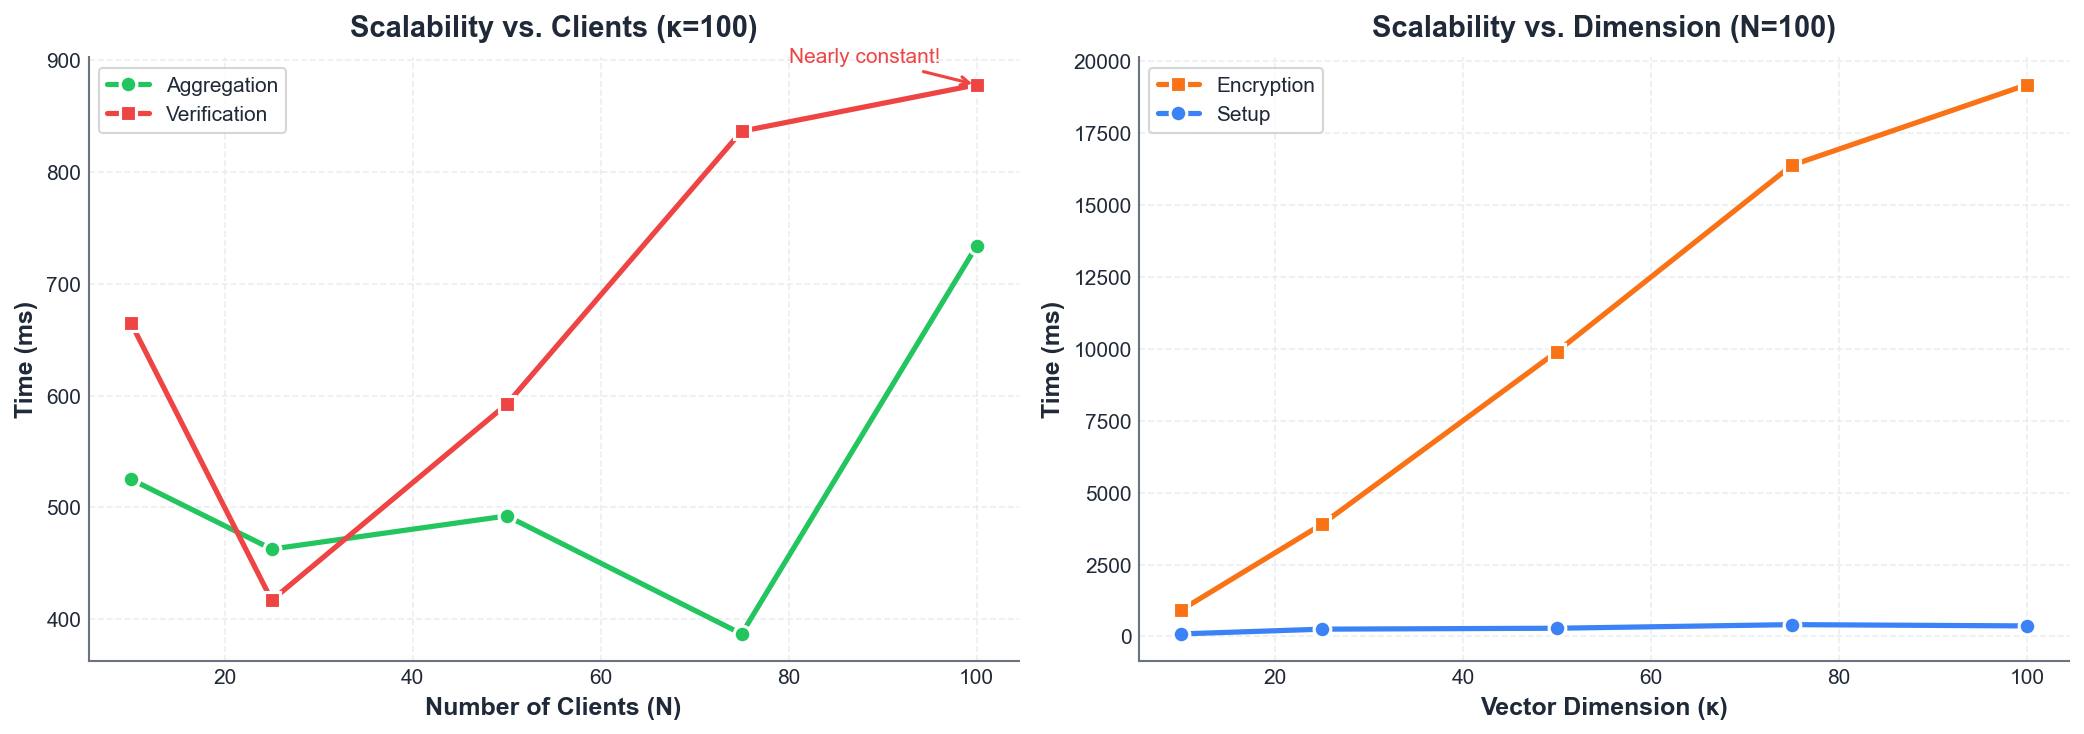
\includegraphics[width=0.65\textwidth]{graph_scalability.png}
    \end{center}

    \vspace{0.2em}

    \begin{columns}[T]
        \begin{column}{0.48\textwidth}
            \textbf{Complexity:}
            \begin{itemize}
                \item Setup: $O(n + \kappa)$ in $\G_2$ multiplications
                \item EncTag: $O(\kappa)$ per user (parallelizable!)
                \item Aggregate: $O(n \cdot \kappa)$ $\G_1$ additions
                \item Verify: $O(n + \kappa)$ pairings
            \end{itemize}
        \end{column}
        \begin{column}{0.48\textwidth}
            \textbf{Key observations:}
            \begin{itemize}
                \item EncTag dominates (bottleneck)
                \item Aggregate nearly constant (DLP $O(1)$)
                \item Verify linear in $n + \kappa$
                \item EncTag is parallelizable across users
            \end{itemize}
        \end{column}
    \end{columns}
\end{frame}

\begin{frame}{Analysis}
    \begin{columns}[T]
        \begin{column}{0.48\textwidth}
            \begin{block}{Strengths}
                \begin{itemize}
                    \item \textbf{Fast aggregation}
                        \begin{itemize}
                            \item DLP table: $O(1)$ lookups
                            \item Nearly constant in $n$
                        \end{itemize}
                    \item \textbf{Public verification}
                        \begin{itemize}
                            \item No secrets required
                            \item Anyone can verify
                        \end{itemize}
                    \item \textbf{Exact results}
                        \begin{itemize}
                            \item No noise (unlike DP)
                            \item Perfect accuracy
                        \end{itemize}
                    \item \textbf{Strong security}
                        \begin{itemize}
                            \item Privacy: CDH
                            \item Verifiability: co-CDH
                        \end{itemize}
                \end{itemize}
            \end{block}
        \end{column}
        \begin{column}{0.48\textwidth}
            \begin{alertblock}{Limitations}
                \begin{itemize}
                    \item \textbf{Encryption cost}
                        \begin{itemize}
                            \item $O(\kappa)$ per user
                            \item Mitigated by parallelization
                        \end{itemize}
                    \item \textbf{DLP table constraint}
                        \begin{itemize}
                            \item $n \times \max < 65536$
                            \item Limits value range
                        \end{itemize}
                    \item \textbf{Trusted setup}
                        \begin{itemize}
                            \item Data Dealer must be honest
                            \item Can be distributed via MPC
                        \end{itemize}
                \end{itemize}
            \end{alertblock}
        \end{column}
    \end{columns}
\end{frame}

% ==============================================================================
% CONCLUSION
% ==============================================================================
\begin{frame}{Conclusion}
    \begin{columns}[T]
        \begin{column}{0.48\textwidth}
            \begin{block}{Implementation}
                \begin{itemize}
                    \item Complete PUDA protocol in Rust
                    \item All four phases functional
                    \item Benchmarked up to 100 clients
                    \item Using Arkworks ecosystem
                \end{itemize}
            \end{block}

            \vspace{0.4em}

            \begin{block}{What I learned}
                \begin{itemize}
                    \item Pairing-based cryptography
                    \item Rust for crypto implementation
                    \item Privacy-preserving protocols
                    \item Performance optimization
                \end{itemize}
            \end{block}
        \end{column}
        \begin{column}{0.48\textwidth}
            \begin{block}{Possible Extensions}
                \begin{itemize}
                    \item Distributed key generation (remove trusted setup)
                    \item Larger DLP tables
                    \item GPU acceleration for EncTag
                    \item Integration with FL frameworks
                    \item Robustness to user dropouts
                \end{itemize}
            \end{block}

            \vspace{0.4em}

            \begin{exampleblock}{Code Summary}
                \begin{itemize}
                    \item Language: Rust
                    \item Library: Arkworks (ark-bls12-381)
                    \item Tested: $n \leq 100$, $\kappa \leq 100$
                \end{itemize}
            \end{exampleblock}
        \end{column}
    \end{columns}
\end{frame}

% ==============================================================================
% THANK YOU
% ==============================================================================
\begin{frame}[plain]
    \vspace{2cm}
    \begin{center}
        {\LARGE\bfseries\textcolor{primary}{Thank You}}\\[15pt]
        \textcolor{accent}{\rule{4cm}{1.5pt}}\\[15pt]
        {\large Questions?}\\[30pt]
        {\small donval@eurecom.fr}
    \end{center}
\end{frame}

\end{document}
